% =============================================================================
% Paper A -- submission draft for Communications Physics (Article)
% Compile: pdflatex + bibtex, or upload to Overleaf as-is.
% NOTE: at submission, switch to the Nature "sn-jnl" template if the
%       editorial screening team asks for it; a clean generic article
%       class PDF with embedded figures is accepted at initial submission.
% All numbers below were recomputed from the raw result files by
% make_paper_figures.py (see paper_a/figures/FIGURE_DATA_LOG.txt).
%
% Revision note 2 (2026-10-07, response to review): the single largest change
% is an ESTIMATOR correction. The residual was reported as the variance of the
% pooled edge-curvature distribution, but the flow is component-wise, so the
% pooled variance contains a between-component term. On every disconnected
% network examined, the within-component variance falls by 3-4 orders of
% magnitude (to 1e-32 in one case) while the pooled value does not: the flow
% DOES uniformise per component, and two of the four "stalled" networks are
% fully accounted for by this. Two connected networks retain a genuine
% within-component residual. This removes the apparent conflict with
% Li-Muench 2026 (J. Funct. Anal. 290, 111367), who prove convergence to
% constant curvature under a connectedness hypothesis that our disconnected
% networks violate.
% Terminology throughout was downgraded to match the evidence: "two fates" ->
% "two regimes"; "constant-curvature floor" -> "operational uniformisation
% threshold"; "geometric limit" -> "consistent with a topology-constrained
% limit"; "family-specific" -> "does not transfer across families"; "surgery
% proves causality" -> "constraint-relaxation control"; "assortativity is
% causal" -> "tracks". V*_G = inf_w Var[kappa(G,w)] is now defined explicitly
% and we state that we do NOT compute it. New controls added: monotonicity
% statistics (variance is empirically near-monotone, not provably so),
% Sinkhorn epsilon sweep, solver-precision probe, independent optimisation /
% root-finding, pooled-vs-within-component decomposition, four-level
% independence hierarchy, sham reported on all 25 pairs as primary.
% corpus divided the per-step variance change by the INITIAL variance, so a
% slow exponential decay was eventually declared saturated (28/28 runs so
% labelled were still falling, median -24.7% over the final quarter). All
% saturation-dependent numbers were recomputed after re-running with a
% corrected criterion (per-step move divided by the CURRENT variance,
% tol 1e-5 for 50 consecutive steps) and, for four networks, with runs of
% 400-912 steps. The headline claim changed: the residual plateau is not a
% universal value near 0.2; the flow splits into a converging and a stalled
% branch. See strict_results/TWO_FATES_REPORT.txt.
% =============================================================================
\documentclass[11pt]{article}
\usepackage[a4paper,margin=2.5cm]{geometry}
\usepackage{amsmath,amssymb}
\usepackage{graphicx}
\usepackage{booktabs}
\usepackage[round]{natbib}
\usepackage[colorlinks=true,linkcolor=blue,citecolor=blue,urlcolor=blue]{hyperref}
\usepackage{microtype}
\graphicspath{{../figures/}}

\newcommand{\kappaedge}{\kappa}
\newcommand{\Var}{\mathrm{Var}}

\title{Finite-time residuals in discrete {Ollivier}--{Ricci} flow:
  a measurement framework, its controls, and its limits}

\author{%
  Qi Fan\thanks{Huaibei Normal University, Huaibei 235000, China.
  e-mail: 8073592@qq.com. ORCID: 0000-0003-3591-3363.}%
  \\ \small Huaibei Normal University, Huaibei 235000, China%
  \\ \small ORCID: 0000-0003-3591-3363}
\date{}

\begin{document}
\maketitle

%------------------------------------------------------------------------------
\begin{abstract}
Discrete {Ricci} flow on a connected weighted graph converges to constant
curvature; what a finite computation sees differs. We separate four quantities
empirical work conflates: the finite-horizon residual $V(T)$, its numerical
counterpart, the trend of $V(t)$, and the geometric infimum $V_G^*$, which we
do not compute. First, the stopping rule used in empirical work normalises the
per-step change of variance by its initial value, which any decaying run
passes: all $28$ runs it labelled saturated were still falling. Second, on a
disconnected graph the pooled variance contains a between-component term that
cannot decay; within components it falls on $34/34$ networks, median factor
$5.7$. Third, under exact transport the residual is step-size converged and
shows negligible decay over the tested $5{,}000$-step horizon;
fixed-$\varepsilon$ regularisation breaks scale invariance. Destroying the
curvature--edge correspondence in a sham control is associated with larger
residuals ($8/8$ families); the structure-to-residual map does not transfer.
\end{abstract}
%------------------------------------------------------------------------------
\section*{Introduction}

Ricci flow deforms a Riemannian metric in the direction of its Ricci
curvature and formed the basis of the uniformisation programme in geometry,
culminating in Hamilton's and Perelman's results on three-manifolds
\cite{Hamilton1982,Perelman2002,Perelman2003}. Its discrete counterpart on
graphs replaces the metric by an edge-weight function and the curvature by a
discrete curvature, most commonly the Ollivier--Ricci curvature
$\kappaedge$ \cite{Ollivier2009,LinLuYau2011}, and updates each edge weight in
the direction of its curvature. ``Graph curvature'' is not a single object:
the Bakry--\'Emery, Ollivier and Forman discretisations disagree on the same
graph \cite{BauerChungLinLiu2017,Sreejith2016,Samal2018,Azarhooshang2020},
and further discretisations exist that are not equivalent to any of them
\cite{SaucanSamalJost2021,Forman2003}, and the Ollivier
curvature itself carries a free idleness parameter
\cite{LinLuYau2011,Bourne2018}; the results below are statements about
\emph{this} curvature and are not expected to transfer to the others. What motivates the geometric reading is that the Ollivier curvature of a
random geometric graph converges to the Ricci curvature of the underlying
manifold \cite{VanderHoorn2023}, in the density regime and for the
neighbourhood radius of that theorem; the one-hop curvature used in network
practice is not the object it controls, and we use it only as context. The
geometric language below is therefore an interpretation of a discrete
construction, not a statement about a recovered manifold. This \emph{discrete Ricci flow} is used for community detection
\cite{Ni2019,LaiBaiLin2022}, graph drawing, network comparison and the analysis
of biological and infrastructural networks
\cite{Sandhu2016,Samal2018,JostLiu2014,GosztolaiArnaudon2021}---the last of
these studies a \emph{dynamical} curvature in which weights diffuse under an
external process, a different evolution from the curvature-driven metric flow
considered here---and sits within the broader programme of describing networks
as geometric objects \cite{Krioukov2010,Boguna2021}.

Two of these results change the update rule or the graph. The continuous-time
normalised flow based on the Ollivier--Lin--Lu--Yau curvature is well posed:
solutions exist and are unique for all times \cite{BaiLinLuWangYau2024}. Very
recently Li and M\"unch proved that the \emph{discrete-time} Ollivier flow
$d_{n+1} = (1-\alpha\kappa_{d_n})\,d_n$ converges to a constant-curvature
metric \emph{under the hypotheses of their theorem}---a finite, connected
(irreducible) weighted graph, exact transport, and an admissible step
size \cite{LiMunch2026}. In the graph-embedding setting
of \cite{Naama2024} a modified flow with a contraction property converges;
flows with \emph{surgery}---deleting or adding edges---converge to constant
curvature on each connected component \cite{MaYang2025}; and for trees the
long-time dynamics of the {Lin}--{Lu}--{Yau} flow have been characterised
directly, including convergence of the normalised tree flow to constant
curvature \cite{BaiLiuLai2026} and a caterpillar-tree characterisation of the
zero-curvature limit \cite{BaiHuaLinLiu2025}; existence, uniqueness, the
directed case and sum-of-curvature identities are likewise settled
\cite{BaiLinLuWangYau2024,BaiHuangLuYau2021,BaiLiLiuLai2025}.

Existing convergence results therefore concern \emph{particular} discrete flow
constructions: a specified update, an exact transport, a fixed admissible edge
set, and hypotheses---connectedness above all---that a third of our corpus
violates. None applies verbatim to the scheme used in the applied literature,
which is multiplicative, entropy-regularised, renormalised every step,
integrated for as long as the budget allows, and applied to graphs that are
frequently disconnected. This paper adds no theorem. Its contribution is a
measurement: a separation of four quantities that empirical work reports
interchangeably (Results), and a set of controls that assign an observed
residual to one of them. Only the last deserves the name ``uniformisation
limit'', and it is not computed here:
\begin{equation}
  V_G^* \;=\; \; \inf_{w:\,E\to\mathbb{R}_{>0}} \Var_E\!\big[\kappa(G,w)\big],
  \label{eq:vstar}
\end{equation}
Nothing below is a lower bound on $V_G^*$. The question is not
\emph{whether} the flow uniformises---under existing hypotheses, it does---but
what a finite computation can be read as saying.

What we find, in outline. The stopping rule used in empirical work is not a
convergence test: all $28$ runs it labelled saturated were still falling. The
pooled variance on a disconnected graph is dominated by a between-component
term that cannot decay, so a third of the corpus looks like a failure when it
is not. Fixed-$\varepsilon$ entropic regularisation breaks the scale
invariance that would license the standard renormalisation as a gauge fixing.
After all of these are controlled, two connected networks from a single family
still relax unusually slowly---a case study, not a demonstration that $V_G^*$
is positive. Homogenisation itself survives every control and depends on the
curvature--edge correspondence ($8/8$ families), while the
structure-to-residual map does not transfer across families. Throughout, the
source family, not the dataset, is the unit of independence
\cite{CameronGelbachMiller2008,MacKinnonNielsenWebb2023}, and results resting
on fewer than five families are labelled exploratory.

Seven controls reversed our own preliminary readings---a plateau near $0.20$
that was a horizon artefact, a community effect that shrank six-fold at
saturation, a spectral-gap hypothesis that failed outright, and the claim that
the per-step renormalisation is a gauge fixing. We report all seven: the
controls, not any single effect, are the transferable part of this work.

%------------------------------------------------------------------------------
\section*{Results}

\subsection*{Analysis populations, evidence tiers, and four quantities that
are routinely conflated}

Ten sample sizes appear below, so we fix them once
(Fig.~\ref{fig:1}a): $C_0$, the $117$ assembled datasets; $C_1$, the $110$
that completed a first-pass run; $C_2$, the $93$ with a complete
structure/variance record---the analysis set, from $17$ source families; $C_3$,
the $80$ long enough to share a common step grid; $C_4$, the $16$ of the
extended strict re-run ($7$ families); and $C_5$, the $9$ re-run under exact
transport ($5$ families).

Two further distinctions organise the evidence. The first is an \emph{evidence tier}: a result is \emph{primary} when it
rests on at least eight independent source families and \emph{exploratory}
when it rests on fewer than five, in which case its $p$-value is an upper bound
on the evidence rather than a measurement of it. The sham control, the
corpus-level component decomposition and the main variance contraction are
primary; the surgery control ($2$ families), the transitivity manipulation
($2$ base graphs) and the assortativity and community sweeps ($4$ base graphs)
are exploratory and are labelled as such.

The second distinction is the one that organises the paper. A number produced
by a finite computation can be any of four things, and empirical work reports
them interchangeably:
\begin{align}
  \text{L1}&\quad V(T): \text{the residual at the horizon we could afford;}
  \nonumber\\
  \text{L2}&\quad V_{\mathrm{num}}(T;\theta): \text{the same, under numerical
  choices } \theta=(\varepsilon,\ \text{solver},\ \Delta t,\ \text{normalisation});
  \nonumber\\
  \text{L3}&\quad \text{the trend of } V(t) \text{ as the horizon } T \text{ grows;}
  \nonumber\\
  \text{L4}&\quad V_G^*\ \text{of Eq.}~(\ref{eq:vstar}),\ \text{a property of the
  graph alone.} \nonumber
\end{align}
Only L4 deserves the name ``uniformisation limit'', and $V(T)\not\Rightarrow
V_G^*$: no residual reported here is a lower bound on it. 

\subsection*{The stopping criterion used in previous work is an operational
diagnostic, not a convergence test}

We first run the Ollivier--Ricci flow ($\alpha=0.5$ idleness, Sinkhorn
transport, $\dot w=-\kappaedge w$) on every network and stop when the
curvature variance $\sigma^2(t)$ stops changing. The rule used in earlier
studies---and in our own first pass---declares saturation when
$|\sigma^2(t)-\sigma^2(t-1)|/\sigma^2(0)$ falls below a tolerance. Under it
$28$ runs were labelled saturated and \emph{all} were still falling---the
variance dropped by a median $24.7\%$ over the final quarter of each run and by
up to $84.9\%$ (Fig.~\ref{fig:2}d). Residuals reported from such runs are
values along a trajectory, not asymptotes.

The reason is worth stating precisely. Suppose $V_t=V_\infty+Ae^{-\lambda t}$.
Then
\begin{equation}
  \frac{|V_t-V_{t-1}|}{V_t}\;\simeq\;
  \frac{A(1-e^{-\lambda})e^{-\lambda t}}{V_\infty+Ae^{-\lambda t}},
  \qquad
  \frac{|V_t-V_{t-1}|}{V_0}\;\simeq\;
  \frac{A(1-e^{-\lambda})e^{-\lambda t}}{V_0},
  \label{eq:stoprate}
\end{equation}
the numerators are the same and both decay, but the denominators are not. With
$V_0$ fixed the ratio decays like $e^{-\lambda t}$ whatever $V_\infty$ is, so
the rule reports elapsed time. With $V_t$ in the denominator the ratio tends to
$1-e^{-\lambda}$ when $V_\infty=0$---it does not tend to zero---and to zero
like $e^{-\lambda t}/V_\infty$ when $V_\infty>0$. The corrected rule is
triggered by runs that are settling onto a positive value and is not triggered
by runs still decaying towards zero. That is the diagnostic we want, and it is
still not a convergence theorem: it says the variance has stopped moving
relative to itself over the observed window, nothing about the limit. We call
it an \emph{operational stopping criterion} throughout, never a convergence
criterion, and every residual below is reported with its horizon. Re-running
population $C_4$ ($n=16$; Methods) under it lowers the median residual from
$0.160$ to $0.109$, in $75\%$ of networks, and the corrected residual spans
five orders of magnitude ($1.9\times10^{-6}$ to $0.51$)---a range no single
\``plateau'' value summarises.
\subsection*{The pooled estimator hides per-component uniformisation}

The residual is conventionally the variance of the pooled set of edge
curvatures. On a disconnected graph the flow acts independently on each
component, so even if every component reaches constant curvature the pooled
variance stops at the dispersion of their limiting curvatures; $34$ of $93$
corpus networks are disconnected, so this is not a corner case. We report two
outcomes: $V_{\mathrm{pooled}}$ (Outcome~A), retained for comparability with
the literature, and $V_{\mathrm{within}}$ (Outcome~B), the primary statistic
for any disconnected network. Writing $m_c$ for the number of edges in
component $c$, $V_c$ for the variance inside it and $\bar\kappa_c$ for its mean
curvature,
\begin{align}
  V_{\mathrm{within}} &= \sum_c \frac{m_c}{m}\,V_c, &
  V_{\mathrm{between}} &= \sum_c \frac{m_c}{m}\,(\bar\kappa_c-\bar\kappa)^2,
  \label{eq:decomp}\\
  V_{\mathrm{pooled}} &= V_{\mathrm{within}} + V_{\mathrm{between}},
  \nonumber
\end{align}
the decomposition is exact at every weight configuration. For a connected graph
$V_{\mathrm{between}}=0$ and the outcomes coincide, so the correction touches
only the disconnected third of the corpus---but there it is decisive (Methods
gives the per-network numbers). The extreme case shows that a nonzero pooled
residual can carry no information about uniformisation at all. Let
$G=G_1\sqcup G_2$ and suppose the flow drives each component to constant
curvature, $\kappa_e=\kappa_i$ on $E_i$, with $\kappa_1\neq\kappa_2$. Then
$V_{\mathrm{within}}=0$ while
\begin{equation}
  V_{\mathrm{pooled}}=\frac{|E_1||E_2|}{(|E_1|+|E_2|)^2}\,(\kappa_1-\kappa_2)^2,
  \label{eq:union}
\end{equation}
which is positive and says nothing about whether the flow succeeded. We verified
Eq.~(\ref{eq:union}) numerically: for $C_5\sqcup C_9$ at unit weights the
curvatures are $0.25$ and $0$, the measured within-component variance is
$0$ to machine precision, and the pooled variance is $1.43495\times10^{-2}$
against the predicted $1.43495\times10^{-2}$ (Supplementary Table~S8).
A graph can therefore be perfectly uniformised within every component and still
report a nonzero pooled residual. 
\begin{table}[t]
\centering
\small
\begin{tabular}{lrrrrrr}
\toprule
Network & comps & steps & $V_{\mathrm{pooled}}$ &
$V_{\mathrm{within}}$ & ratio & between \\
 & & & (end) & (end) & $V_w/V_w(0)$ & share \\
\midrule
kilifi  & 2 & 250 & $1.40\times10^{-2}$ & $5.83\times10^{-6}$ & $1.8\times10^{-4}$ & 100.0\% \\
oman    & 5 & 250 & $1.97\times10^{-2}$ & $1.78\times10^{-5}$ & $1.4\times10^{-3}$ & 99.9\% \\
ksa     & 8 & 183 & $5.80\times10^{-3}$ & $9.11\times10^{-33}$ & --- & 100.0\% \\
hw      & 4 & 65  & $4.29\times10^{-2}$ & $1.71\times10^{-3}$ & $1.0\times10^{-1}$ & 96.0\% \\
\midrule
g106    & 1 & 150 & $2.38\times10^{-2}$ & $2.38\times10^{-2}$ & $3.8\times10^{-1}$ & 0.0\% \\
g105    & 1 & 115 & $1.30\times10^{-2}$ & $1.30\times10^{-2}$ & $3.1\times10^{-1}$ & 0.0\% \\
\bottomrule
\end{tabular}
\caption{\textbf{Pooled versus within-component curvature variance.} For every
disconnected network of $C_4$ the within-component variance falls by one to
three orders of magnitude while the pooled variance does not: the flow has
uniformised each component and the estimator reports their disagreement. The
two connected networks at the bottom are shown for contrast---for them the
decomposition is trivial. Horizons differ because each run had a wall-clock
budget, so the connected residuals are finite-horizon values, not bounds.}
\label{tab:components}
\end{table}

Over the corpus rather than the strict sample the picture changes
quantitatively. Across all $34$ disconnected networks the within-component
variance falls in $34/34$, but by a median factor of only $5.7$
(interquartile range $2.2$--$10$), exceeding $10^{2}$ on two networks, with
final values spanning $1.9\times10^{-32}$ to $8.1\times10^{-2}$
(Supplementary Table~S3); the between-component term accounts for a median
$65\%$ of the pooled variance and more than half of it on $22$ of $34$. The
direction is universal; the magnitude on which we earlier based the
claim---three to four orders of magnitude---is the behaviour of the two most
extreme networks, not the typical one, and we withdraw it.

Two of the four Pattern~II networks (\texttt{kilifi}, \texttt{oman})
are disconnected, and for both the near-plateau is fully accounted for
by this term: on those two the flow did not fail. The two that
remain---\texttt{ENZYMES\_g105} and \texttt{ENZYMES\_g106}---are connected,
so their residual is within-component and is not an estimator artefact.

We treat these two as \emph{case studies}, not as evidence about connected
networks in general: two graphs from one family out of seventeen support no
prevalence claim. Under every numerical control we applied---exact transport, a
scale-equivariant schedule, a ten-fold range of step size, a $5{,}000$-step
horizon and two independent optimisers---they exhibited unusually slow
relaxation. We have not computed $V_G^*$, so this is consistent with a
topology-constrained limit and does not establish that the infimum is
positive; it is equally consistent with a metastable transient longer than any
horizon we could afford.
\subsection*{Two finite-horizon relaxation patterns}

Subject to that correction the remaining spread separates into two behaviours
(Fig.~\ref{fig:2}e,f). Classifying each run by its decay rate over the final
quarter, $11$ networks show Pattern~I (continued relaxation): the residual keeps
falling at a median $-5.5\times10^{-3}$ per step and has reached a median of
$0.024$. Four show Pattern~II (near-plateau over the observed horizon): the
decay decelerates below $10^{-4}$ per step and the residual sits at a median of
$0.17$ ($0.154$--$0.238$); one is undecided. Two of the four are the
disconnected networks explained above. These are descriptions of what happened
inside a horizon, not claims about limits.

Because a rate estimated in one window says nothing about the next, we also
report the rate trajectory. Figure~\ref{fig:8} plots the local relaxation rate
$r_t=-\log(V_t/V_{t-1})$ for all $16$ runs of $C_4$: $r_t>0$ is decay,
$r_t\approx0$ a plateau, $r_t<0$ a rebound. The patterns appear as two
bands; the $10^{-3}$ per step line between them is a descriptive threshold,
not a theoretical boundary: runs cross it, so it carries no information about
the limit. What separates the patterns is the state of the weights: Pattern~II
networks end with a weight span of median $2.8\times10^{5}$ against
$3.9\times10^{2}$ (Mann--Whitney $p=0.039$ at network level). This is the
number most exposed to clustering: the family-level bootstrap interval is
$[2.64,5.25]$ decades, but dropping any single family moves the network-level
$p$ to $0.017$--$0.105$. We report the separation as an association that
survives clustering in magnitude but not in significance, and claim no
mechanism---a diverging weight span is also what makes the transport subproblem
ill conditioned.

\subsection*{The regularised curvature is not scale invariant---and the
residual survives that being fixed}

In Pattern~II the weights span $10^{5}$--$10^{11}$, so the transport cost
matrices are badly scaled and the entropy-regularised Sinkhorn surrogate is at
its weakest: a residual measured there could be an artefact of the
regularisation strength, the solver tolerance or floating-point resolution
rather than a property of the graph. We ran five controls; the first uncovered
an error in our own framing.

\emph{Scale invariance.} For the exact curvature
$\kappa(G,cw)=\kappa(G,w)$, which is what would license the per-step
renormalisation as removal of a null direction. For the entropy-regularised
cost this fails: with $\varepsilon$ fixed, $C\mapsto cC$ changes the kernel
$\exp(-C/\varepsilon)$ and hence the plan. We measured the violation on nine
networks and six rescaling factors (Methods): under exact $W_1$ and under a
scale-\emph{equivariant} schedule $\varepsilon_t\propto s_t$ the curvature is
invariant to machine precision, while under the fixed-$\varepsilon=0.05$
solver used elsewhere in the paper $\max_e|\kappa_e(cw)-\kappa_e(w)|$ reaches
$1.40$ at the initial weights and $3.86$ after $150$ steps. The claim in our
previous version---that the renormalisation removes a null direction---is
therefore false as stated, and we withdraw it; $\sum_e\log w_e=0$ in the
independent optimisation below is a normalisation of the search space, not a
gauge fixing.

Two things bound the damage: $s_t$ drifts by only $0.98$--$1.29\times$ over
$200$ steps because the mean weight is renormalised every step, so the
violation does not compound; and repairing it barely changes the numbers. Under
the scale-equivariant schedule at a matched horizon of $200$ steps the pooled
residual moves by a median $-4.6\%$ (at most $-14\%$) with no change of
ordering, and replacing regularised transport by exact transport
\emph{raises} the residual on the two connected networks ($+5\%$ on
\texttt{g105}, $+193\%$ on \texttt{g106})---slower relaxation, not a lower
floor. The conclusion survives the repair; only the interpretation had to go.

\emph{Exact transport at a long horizon.} Running population $C_5$ with exact
$W_1$ transport for $2{,}000$ steps separates the networks cleanly
(Fig.~\ref{fig:3}c; Methods gives the values): five reach a within-component
variance below $10^{-11}$---two connected and three disconnected, the latter
with a pooled variance of $0.033$--$0.112$ that is entirely
between-component---and four do not, among them the three connected ENZYMES
graphs. Both halves of the story survive exact transport.

\emph{Extended horizon.} Extending the three connected ENZYMES runs from
$2{,}000$ to $5{,}000$ steps under exact transport changes their residual by
$+0.009\%$ (\texttt{g105}), $+0.0002\%$ (\texttt{g106}) and $+0.17\%$
(\texttt{g10}), while the weight span grows to $2\times10^{71}$
(Supplementary Table~S7). Over three thousand further steps of an unregularised
solver these networks show no appreciable decay---evidence about the
trajectory, not about the infimum.

\emph{Step size at fixed physical time.} Holding physical time fixed at $T=20$
and varying $\Delta t$ ten-fold, from $0.01$ ($2{,}000$ steps) to $0.1$ ($200$
steps) under exact transport on $C_5$, the residual at $T$ changes by at most
$0.05\%$ on the seven networks that have not converged by then and by at most
$4.9\%$ on the two that have converged by then
(Supplementary Table~S7): not a time-discretisation artefact.

\emph{Regularisation strength.} Entropic smoothing shrinks curvature
magnitudes, and could hide or invent a spread. Re-run at a \emph{matched}
horizon---the stopping step itself moves with $\varepsilon$---over a
$20$-fold reduction of $\varepsilon$ with periodic exact-transport
checkpoints, the exact-transport residual spans $5.1\%$ on \texttt{g105}
and $9.7\%$ on \texttt{g106}. Where the estimators disagree, {Sinkhorn} is
\emph{below} exact, by $3.6\times$ on \texttt{g106}, so the artefact hides
the residual; at $\varepsilon=0.002$ the solve fails and we exclude those
runs (Supplementary Table~S9).

No observed residual is claimed to bound $V_G^*$.

\subsection*{The plateau is associated with the curvature--edge
correspondence}

A plateau could, in principle, be a mechanical artefact of the update rule
$w \leftarrow w\,e^{-\Delta t\,\kappaedge}$ with renormalisation, rather than
a property of the geometry. We therefore ran a \emph{sham flow}: identical
numerics, but at every step the curvature values are randomly permuted across
edges before the update (Methods). If homogenisation were mechanical, the sham
arms would homogenise too. They do not. These $25$ pairs are not $25$ independent
experiments: they come from $8$ source families. At the network level the split
is $24/25$ (Methods); aggregating within family and testing across families,
all $8/8$ families show the sham arm higher
(sign test $p = 3.9\times10^{-3}$; family-level sign-flip permutation
$p = 3.9\times10^{-3}$; cluster-bootstrap $95\%$ interval for the median
log-ratio gap $[-2.60, -0.69]$, excluding zero), and the worst
leave-one-family-out $p$ is $9.2\times10^{-4}$
(Fig.~\ref{fig:2}c, Methods). The effect size is unchanged---a median factor
of $2.6$---but the evidence is that of $8$ clusters, not $25$ networks. Destroying the
curvature--edge mapping does not merely slow the flow; it suppresses
homogenisation over the tested horizon, by a median factor of $2.6$. The
homogenisation we observe is therefore \emph{associated with} the geometric
correspondence between edge curvature and edge update, and is not reproduced by
the update rule alone when that correspondence is randomly destroyed. The
control randomises the pairing and the spatial arrangement together, so it
shows the correspondence matters under this intervention, not that no other
mechanism could.

\subsection*{Relaxing the edge-set constraint largely removes the residual}

Surgery-based discrete Ricci flows converge to constant curvature by deleting
edges \cite{MaYang2025}. Our counterpart control asks the converse question:
how much of the residual is due to edges the flow is not allowed to remove?
In paired runs with identical numerics, removing only the edges whose
curvature stays above a fixed tolerance ($4$--$14$ edges of $41$--$84$, with
bridge edges protected) and re-running the flow collapses the residual in
$5/5$ defensible pairs (one-sided sign test $p = 0.031$; Fig.~\ref{fig:4}), by
a median factor of $6.6$ and up to $132\times$. The five pairs come from only
two families (four ENZYMES, one \texttt{scc\_rt}), so the family-level test has
essentially no power: both families show the relaxed arm lower, but with two
clusters a sign test cannot go below $p = 0.25$. The direction is consistent
in every family (median drop $25\times$ within ENZYMES, $1.05\times$ for the
single \texttt{scc\_rt} pair); the magnitude is not established at family
level, and the network-level $p = 0.031$ should be read as an upper bound on
the evidence.

This is a \emph{constraint-relaxation} control, not a causal demonstration:
the intervention is outcome-informed and bridges are protected by fiat. The
defensible claim is that the residual measures how far a graph is from constant
curvature \emph{if its edge set may not change}---which makes our result
complementary to, rather than in conflict with, the surgery literature, whose
flows destroy exactly this quantity.

\subsection*{In controlled rewiring, transitivity changes the relaxation
time, not the endpoint}

Why do some networks homogenise almost completely while others retain a large
residual at the same horizon? We manipulated single structural quantities on
synthetic graphs while holding the degree sequence exactly fixed, using
degree-preserving double-edge swaps \cite{MaslovSneppen2002} (Methods).
Raising transitivity from $0.12$ to $0.43$--$0.46$---the transitivity of the
median real network---raises the residual at a matched horizon of $250$ steps
by three orders of magnitude on both base graphs. Followed to terminal states,
both arms of the first graph reach the operational uniformisation threshold, at
step $381$ (low transitivity) and $884$ (high), and the fold between them
collapses from $31\times$ at $125$ steps to $1.02$ at $900$
(Fig.~\ref{fig:5}b,c). The effect is therefore entirely a difference in time
scale: the arms end in the same state and differ only in arrival time
($2.3\times$ in steps), because the high-transitivity arm decays slowly then
accelerates $11$-fold. Nothing measured in one window predicts the next. Within
the tested design, transitivity was the structural variable most clearly
associated with the observed relaxation-time difference, while the assortativity
change carried along with it accounts for only $2.5$--$3.4\%$ of the effect.
Two earlier readings are withdrawn: that transitivity raises the
\emph{plateau} by $25$--$37\times$, and that it selects a relaxation pattern.
Both were horizon artefacts. The manipulation rests on two base graphs and is
\emph{exploratory}. The assortativity and community sweeps (Methods) are
secondary: both ran under the unsafe stopping rule, and at saturation the
community effect shrinks from $6.1\times$ to $1.35\times$.

\subsection*{The structure-to-residual mapping does not generalise across
families}

Transitivity and assortativity correlate with the residual within bases and
within the largest family in our corpus (ENZYMES, $n=15$ converged:
$\rho = +0.73$ for transitivity, $p = 0.002$). But the correlation is
\emph{not} a predictor. In leave-one-family-out cross-validation across 25
networks, only assortativity rises even marginally above the intercept
baseline, and it still explains essentially none of the variance
(Fig.~\ref{fig:6}a): assortativity reaches out-of-sample $R^2 = +0.04$
against a baseline of $-0.17$, modularity reaches $-0.11$, and the
four-variable model $-0.79$. Within ENZYMES the transitivity correlation collapses once
size is controlled (partial $\rho = +0.25$, $p = 0.37$, with size itself at
$\rho = -0.76$), and at the family level the trend is positive but not
significant ($5$ families, $\rho = +0.50$, $p = 0.39$;
Fig.~\ref{fig:6}b). The relation between global structure and the residual is
\emph{ecological}: it holds between families rather than within them, and it
does not transfer. This is a null result and we regard it as one of the main
findings. An out-of-sample $R^2$ below the intercept baseline is evidence that
\emph{these models do not transfer}, not that the residual is intrinsically
family-specific; the latter would require showing that no statistic predicts
it. Of the descriptive correlations reported alongside the test, assortativity
($\rho=+0.41$) survives family-level resampling ($95\%$ interval
$[+0.18,+0.72]$) and transitivity ($\rho=+0.22$) does not
($[-0.30,+0.55]$; Fig.~\ref{fig:6}c): in-sample associations should be read
with the family, not the network, as the unit.

\subsection*{No evidence that the initial spectral gap predicts early decay}

Finally, the dynamics. Curvature controls eigenvalue estimates \cite{LinYau2010},
so the spectral gap is a natural candidate predictor. The early decay rate of the curvature
variance is uncorrelated with the spectral gap of the initial Laplacian across 41
usable units spanning three orders of magnitude in $\lambda_1$
($\rho = -0.03$; $|{\rho}| \ge 0.31$ detectable at $\alpha=0.05$), and in a
joint model the gap carries no information beyond size and mean degree
($\beta = -0.10$, $p = 0.18$), while mean degree dominates
($\beta = +0.70$, $p = 3\times10^{-4}$;
Fig.~\ref{fig:7}a). This null is robust to clustering: over the $11$ families
the cluster-bootstrap interval for $\rho$ is $[-0.43, +0.39]$, and the sign is
stable in only $58\%$ of replicates. We report this as the negative result it
is: in this sample we find no evidence that the initial spectral gap predicts the
observed early decay rate. It does not
follow that mean degree is the causal driver---a regression coefficient on
observational network data is not an intervention---and we do not claim it.
What the rate tracks is where the flow is at the end of the run
($\rho=-0.43$; partial $\rho=-0.63$ controlling for size and mean degree;
Fig.~\ref{fig:7}b). At the network level this is significant
($p=1\times10^{-5}$), but the family-level interval is $[-0.68,+0.16]$ and
includes zero, so we withdraw our earlier formulation of it as a result. Part of
the association is definitional in any case: the fitted rate and the final
variance are two summaries of the same trajectory.

%------------------------------------------------------------------------------
\section*{Discussion}

Four statements survive the controls above. We give them in order of
evidential strength, and each is stated at the level the evidence supports.

\emph{1. A finite-time residual is not a convergence certificate.} The
stopping rule used in empirical work divides the per-step change of the
variance by its initial value; Eq.~(\ref{eq:stoprate}) shows that this ratio
decays like $e^{-\lambda t}$ whatever the limit is, so the rule reports
elapsed time. All $28$ runs it labelled saturated were still falling. What we
use instead is an \emph{operational stopping criterion}: the variance has
stopped moving relative to itself over the observed window. It is a better diagnostic and still not a
convergence theorem; every residual here is reported with its horizon.

\emph{2. On a disconnected graph the pooled curvature variance can
substantially overstate within-component non-uniformity.} The decomposition of
Eq.~(\ref{eq:decomp}) is exact, and Eq.~(\ref{eq:union}) exhibits the case
$V_{\mathrm{within}}=0$ with $V_{\mathrm{pooled}}>0$: a graph can be perfectly
uniformised within every component and still report a nonzero residual. Across
all $34$ disconnected networks of the analysis set the within-component
variance falls, by a median factor of $5.7$; our earlier claim of three to
four orders of magnitude on every disconnected network is withdrawn. A third of the corpus is disconnected and the pooled
variance is the standard reporting choice, so this correction applies to
previous empirical work as much as to our own.

\emph{3. Entropic transport regularisation changes the numerical curvature
dynamics unless its scale is controlled.} With $\varepsilon$ held fixed the
regularised curvature is not invariant under $w\mapsto cw$, so the usual
reading of the per-step renormalisation as a gauge fixing is unavailable and
we withdraw it. Exact transport and a scale-equivariant schedule restore
invariance, and the residual survives both. Nor is it a regularisation or discretisation artefact: at a matched
horizon it moves by $\le9.7\%$ over a $20$-fold $\varepsilon$ reduction and
by $\le0.05\%$ over a ten-fold $\Delta t$ range at $T=20$.

\emph{4. After these controls some connected networks still relax very slowly,
but the present evidence does not establish a positive geometric infimum.} Two
connected ENZYMES networks---two graphs from one family of seventeen---showed
no appreciable decay over $3{,}000$ further steps of exact transport, to a
$5{,}000$-step horizon, while their weight span grew to $10^{71}$. We treat it as a case study. We have not computed $V_G^*$, nothing here bounds it, and the
observation is equally consistent with a metastable transient longer than any
horizon we could afford. The correct description is \emph{unexplained by the
tested controls}, which is strictly weaker than \emph{intrinsic geometric
obstruction}.

Homogenisation itself is not in doubt, and it is tied to the
curvature--edge correspondence: destroying that correspondence in the sham
control is associated with suppressed homogenisation in $8/8$ families---an
association under one intervention, not a proof of necessity. What remains unpredicted is which real networks relax quickly. The
structure-to-residual map does not transfer across families; transitivity moves
the relaxation time and not the endpoint; and a decay rate measured in one
window carries no information about the next, which is why
Fig.~\ref{fig:8} reports the rate trajectory rather than a classification.

Table~\ref{tab:assumptions} sets out, hypothesis by hypothesis, why the
convergence theorem most relevant to us does not transfer to the scheme studied
here. It is a statement about the hypotheses, not a criticism of the theorem:
where the hypotheses hold---on connected graphs, under exact transport---we
observe what the theorem predicts. The remaining differences---exponential
versus Euler update, regularised versus exact transport---we tested directly
rather than leaving them open (Methods). Neither produces the residual: at the
matched step size the two updates agree within a factor of three on all seven
networks tested, and at fixed physical time the exponential flow with exact
transport has not collapsed.

\begin{table}[t]
\centering
\begin{tabular}{p{2.6cm}p{3.0cm}p{3.0cm}}
\toprule
Hypothesis / ingredient & Li~\&~M\"unch \cite{LiMunch2026} & Scheme used here \\
\midrule
Graph & finite, weighted, connected (irreducible) & finite, weighted; $34$ of $93$ disconnected \\
Curvature & exact {Ollivier} $W_1$ & entropy-regularised {Sinkhorn}, $\varepsilon=0.05$ \\
Update & $d_{n+1}=(1-\alpha\kappa)d_n$ & $w_e\leftarrow w_e e^{-\Delta t\,\kappa_e}$, $\Delta t=0.05$ \\
Renormalisation & not part of the statement & mean weight renormalised every step \\
Step size & admissible range & fixed; $\alpha=0.5$ and $0.05$ both tested \\
Edge set & fixed, no surgery & fixed; surgery arm adds a control only \\
\bottomrule
\end{tabular}
\caption{\textbf{Why the convergence theorem does not transfer.} The theorem is
used here as a reference point, not as a prediction: each row is an ingredient
on which the scheme studied differs from the one proved to converge. Section
\emph{Exact transport to a long horizon} restores two of these ingredients
(exact curvature, ten-fold horizon) and reports what changes.}
\label{tab:assumptions}
\end{table}
For practitioners: stop when the variance stops moving relative to
\emph{itself}; \emph{report the within-component variance whenever the
graph is disconnected}, since the pooled variance makes a uniformised network
look like a failure; with a fixed-$\varepsilon$ solver, report the effective ratio
$\varepsilon/s_t$ or use a scale-equivariant schedule; do not treat the
residual as predictable across families, nor networks from one source as
independent replicates.

\emph{Limitations.} Population $C_4$ covers $16$ networks because a step costs
$0.03$--$12$~s and the corpus would need $\sim80$~h to take all $93$ to $400$
steps; the sample is cost-stratified, not random, and biased towards small
graphs. Four further limitations bear on the claims. \emph{(i) Estimator.}
$V_{\mathrm{pooled}}$ and $V_{\mathrm{within}}$ are not interchangeable on a
disconnected graph; both are reported for every network, and the
within-component re-run reached a median of only $86$ steps, so those residuals
are themselves finite-horizon quantities. \emph{(ii) Transport.} The curvature
is a Sinkhorn surrogate at fixed $\varepsilon$=0.05 and idleness $\alpha$=0.5; the
extreme weight ratios reached in Pattern~II make the transport subproblem ill
conditioned, and we have tested but not eliminated a regularisation or
precision origin for the residual. \emph{(iii) Independence.} The unit of
independence is the source family, and within the synthetic sweeps the base
graph---two of which is not a basis for a general claim. \emph{(iv)
Attribution.} The manipulations hold the degree sequence fixed but not motif
structure, shortest paths or spectra, and the assortativity and community
sweeps inherit the unsafe stopping rule, so their magnitudes carry horizon
bias. A lower bound on $V_G^*$ in terms of a conflict between
curvature-feasible intervals is conjectured, not proven.
%------------------------------------------------------------------------------
\section*{Methods}

\paragraph{Corpus.} We assembled 117 weighted-network datasets from a public
network repository, covering 12 domains (cheminformatics, animal social
networks, dynamic contact networks, temporal reachability, biological,
brain, power, interaction, web, ecology, infrastructure and economic
networks). 110 runs completed. The analysis set comprises the 93 networks
with a complete structure/variance record; 17 runs were excluded (degenerate
initial curvature variance at float-noise level, or runs that could not
start/complete for size or load reasons). Within it, 41 runs satisfy the
convergence criterion below; a stricter tail-drift test leaves 31. The
analysis set spans $n=4$ to $6{,}809$ nodes (median 52) and 17 source
families (11 with $\ge 3$ networks); 34 of 93 networks are disconnected.
Supplementary Table~S1 lists every dataset with its exclusion status.

\paragraph{Flow.} Ollivier--Ricci curvature with idleness $\alpha=0.5$,
optimal transport computed by entropic-regularised Sinkhorn iterations
(regularisation $\varepsilon=0.05$)
\cite{Sinkhorn1964,SinkhornKnopp1967,Cuturi2013,PeyreCuturi2019}. Each step applies
$w_e \leftarrow w_e \exp(-\Delta t\, \kappaedge_e)$ with $\Delta t = 0.05$,
followed by renormalisation of the mean weight to $1$. Edge weights act as
edge lengths. \emph{This is a normalised, entropy-regularised discrete Ricci
flow, not an exactly scale-invariant Ollivier--Ricci flow}: with $\varepsilon$
held fixed the curvature is not invariant under $w\mapsto cw$ (Results), so
the per-step renormalisation is a constraint on the state and not the removal
of a null direction, and no result here should be read as a statement about
the exact flow unless it is explicitly derived from the exact-transport
re-runs described below. Three variants of the same scheme are run as
controls: \emph{exact transport}, in which every transport problem is solved
by network simplex (POT \texttt{ot.emd}, with a HiGHS linear-programming
fallback) so that $\kappa_e = 1-W_{1,e}/d_e$ is the exact Ollivier curvature;
\emph{scale-equivariant regularisation}, in which
$\varepsilon_t = \varepsilon_0\, s_t/s_0$ with $s_t$ the mean entry of the
transport cost matrices at step $t$, which restores exact equivariance; and
the \emph{first-order Euler update} $d_e\leftarrow(1-\alpha\kappa_e)\,d_e$
studied by \cite{LiMunch2026}, run with and without the mean-weight
renormalisation and with $\alpha\in\{0.05,0.5\}$, so that the only difference
from the production scheme is the update rule. Initial weights follow dataset metadata: where a dataset
supplies positive edge weights they are interpreted as lengths
(\texttt{weight\_mode = auto} with the \texttt{distance} convention), and
where the dataset is unweighted or carries non-positive weights---the majority
of the corpus---every edge is initialised to unit length. ``Weighted
network'' in this paper therefore refers to the \emph{evolving} weight
function, not to an assumption that the source data carry physical weights.
Runs use a step horizon and a wall-clock budget, whichever is reached first;
per-step trajectories are stored.

\paragraph{Sample sizes.} \emph{Further numerical controls.} Re-running the flow with
$\varepsilon\in\{0.1,0.05,0.02,0.01\}$ leaves the residual on
\texttt{kilifi} invariant to $0.9\%$ ($0.1771$--$0.1788$ at $250$ steps) and
\emph{raises} it on the other three (\texttt{oman} $0.170\to0.235$,
\texttt{g106} $0.175\to0.529$, \texttt{ksa} $0.146\to0.964$), in each case
with a smaller weight span at the same horizon: slower relaxation, not a higher
plateau. The residual does not vanish as the regularisation is removed. This is
not simply the finite-$\varepsilon$ bias of the transport cost relative to exact
$W_1$, which is a separate and well-studied quantity
\cite{Genevay2019,Feydy2019,Janati2020,Schmitzer2019}: debiased formulations, stabilised
$\varepsilon$-scaling and sparse exact schemes address different aspects of that
bias, and we do not claim to have removed it. What we observe is a property of
the trajectory---the horizon at which the residual is read moves with
$\varepsilon$. Tightening the solver from $\text{tol}=10^{-9}$ to $10^{-13}$
and from $5\times10^3$ to $5\times10^4$ iterations moves the variance by
$3\times10^{-5}$ to $2\times10^{-2}$. Two searches of a different algorithmic
class from the flow (a trust-region solver for the uniformisation equations
$\kappa_e(w)-\bar\kappa(w)=0$, and multi-start quasi-Newton minimisation of
$\Var[\kappa]$ over $\log w$) found, under a matched wall-clock budget, no
weighting of lower variance than the flow on five of six networks; on
\texttt{kilifi} they agreed with it to $2\%$ ($0.177$, $0.180$) and
neither solved the equations
($\max_e|\kappa_e-\bar\kappa|=1.3\times10^{-2}$). No weighting with
substantially lower variance was found; we make no claim that any observed
residual bounds $V_G^*$. (Full descriptions are in Methods.)

\paragraph{Two experimental stages.} The corpus screening (110 datasets,
10 steps, $t=0.5$) and the long-run study (16 networks re-run to
400--912 steps) are separate experiments and are reported as such. The
10-step stage establishes only that curvature heterogeneity falls in the
transient; every statement about long-time behaviour comes from the second
stage. In particular, the first stage's 10-step horizon sits at $V=0.781$ of
the initial variance on the median trajectory, which is a transient, not a
result.

\paragraph{Convergence.} Two stopping rules are used, and the difference
between them is one of the results. The \emph{initial-variance} rule, used for
the first corpus pass and in earlier studies, stops when
$|\sigma^2(t)-\sigma^2(t-1)|/\sigma^2(0) < 10^{-4}$ for a fixed window;
because the denominator is constant while the numerator decays, any
exponentially decaying run eventually satisfies it (28/28 runs so labelled in
our corpus were still falling, median $-24.7\%$ over the final quarter). The
\emph{current-variance} rule used for the strict re-run stops when
$|\sigma^2(t)-\sigma^2(t-1)|/\sigma^2(t) < 10^{-5}$ for 50 consecutive steps.
This is a statement about the window just observed and nothing else: it does
not bound the future, and we draw no such inference from it. We therefore
report the terminal window explicitly rather than extrapolate it
(Supplementary Table~S10). Over the final $50$ steps of the $16$ strict runs,
the per-run median of $r_t$ has median $4.7\times10^{-3}$ per step across runs
and ranges from $-3.3\times10^{-5}$ to $1.7\times10^{-2}$; $14$ of $16$ runs
have a terminal median rate above $10^{-4}$ per step, and---the observation
that most directly falsifies any forward extrapolation---two runs have a
\emph{negative} terminal median rate, i.e. their variance was rising at the
end of the run. The realised relative change of $V$ over the same final window
is $21\%$ in magnitude on the median run and up to $58\%$. A small change over
fifty steps is therefore a description of those fifty steps. Runs that exhaust the horizon
or the wall-clock budget while still falling are flagged \emph{still falling},
and runs that meet the rule are called \emph{operationally stopped} or
\emph{near-plateau at the observed horizon}---never \emph{converged}.

Two qualifications accompany the rule. First, monotonicity of the variance is
\emph{assumed}, not proven: we verified empirically that $10$ of the $16$
strict trajectories never increase; that the remaining six do so on at most
$16.3\%$ of steps ($234$ of $6{,}052$ increments) with a maximum single
increase of $0.39\%$ of the current value; and that the cumulative upward
movement is at most $3.7\%$ of the total decrease achieved. Because the
criterion fires on $|\Delta V|$ rather than on its sign, these violations do
not affect any regime assignment, but the last observed value of a truncated
run is treated as a finite-horizon residual, not as a rigorous upper bound on
the asymptotic value. Second, as $V\to 0$ the relative criterion's
denominator also tends to zero, so we additionally monitor the absolute
increment $|\sigma^2(t)-\sigma^2(t-1)|$; every run reported as having reached
the operational uniformisation threshold ($V \le 10^{-6}$ of the initial
variance) also has an absolute increment below $10^{-9}$ in variance units,
i.e.\ it is far from the regime where the relative test is numerically
vacuous. Sixteen networks were re-run under the strict rule; per-network step
counts, residuals, decay rates and weight spreads are given in Supplementary
Table~S2.

\paragraph{Variance decomposition.} For every run we record the component
label of each edge and decompose the pooled curvature variance as in
Eq.~\eqref{eq:decomp}, where $c$ indexes connected components, $m_c$ is the
number of edges in component $c$ and $\bar\kappa_c$ its mean curvature. Both
terms are evaluated at the same weight configuration as the pooled value, so
the decomposition is exact. For a connected graph the decomposition is trivial
($V_{\mathrm{within}}=V_{\mathrm{pooled}}$); we therefore re-ran the
disconnected networks of the analysis set to the horizon each reached in the
first pass (capped at $200$ steps and $900$~s of wall clock). All $34$ completed, and both
outcomes are reported for every one of them (Supplementary Table~S3). The corpus-level
statistics quoted in this paper use $V_{\mathrm{pooled}}$ for connected
networks and $V_{\mathrm{within}}$ for disconnected ones.

\paragraph{Scale-invariance probe.} On nine networks (the four
Pattern~II runs and five controls) we evaluate the curvature at the
current weights, then multiply every edge weight by
$c\in\{0.25,0.5,2,4,10,100\}$ and re-evaluate, reporting
$\max_e|\kappa_e(cw)-\kappa_e(w)|$ and the change in $\Var[\kappa]$. The probe
is run at the initial weights and after $150$ flow steps, and separately for
the three transport backends (fixed-$\varepsilon$ Sinkhorn, scale-equivariant
Sinkhorn, exact $W_1$). The cost scale $s_t$ is recorded at every step of
every run, which is what makes the drift of the effective ratio
$\varepsilon/s_t$ measurable (Supplementary Table~S6).

\paragraph{Numerical controls.}
\emph{Further numerical controls.} Re-running the flow with
$\varepsilon\in\{0.1,0.05,0.02,0.01\}$ leaves the residual on
\texttt{kilifi} invariant to $0.9\%$ ($0.1771$--$0.1788$ at $250$ steps) and
\emph{raises} it on the other three (\texttt{oman} $0.170\to0.235$,
\texttt{g106} $0.175\to0.529$, \texttt{ksa} $0.146\to0.964$), in each case
with a smaller weight span at the same horizon: slower relaxation, not a higher
plateau. The residual does not vanish as the regularisation is removed. This is
not simply the finite-$\varepsilon$ bias of the transport cost relative to exact
$W_1$, which is a separate and well-studied quantity
\cite{Genevay2019,Feydy2019,Janati2020,Schmitzer2019}: debiased formulations, stabilised
$\varepsilon$-scaling and sparse exact schemes address different aspects of that
bias, and we do not claim to have removed it. What we observe is a property of
the trajectory---the horizon at which the residual is read moves with
$\varepsilon$. Tightening the solver from $\text{tol}=10^{-9}$ to $10^{-13}$
and from $5\times10^3$ to $5\times10^4$ iterations moves the variance by
$3\times10^{-5}$ to $2\times10^{-2}$. Two searches of a different algorithmic
class from the flow (a trust-region solver for the uniformisation equations
$\kappa_e(w)-\bar\kappa(w)=0$, and multi-start quasi-Newton minimisation of
$\Var[\kappa]$ over $\log w$) found, under a matched wall-clock budget, no
weighting of lower variance than the flow on five of six networks; on
\texttt{kilifi} they agreed with it to $2\%$ ($0.177$, $0.180$) and
neither solved the equations
($\max_e|\kappa_e-\bar\kappa|=1.3\times10^{-2}$). No weighting with
substantially lower variance was found; we make no claim that any observed
residual bounds $V_G^*$. (Full descriptions are in Methods.)

\paragraph{Numerical controls.}
\emph{Regularisation sweep:} the flow is re-run on both Pattern~II networks
(\texttt{g105}, \texttt{g106}) with
$\varepsilon\in\{0.1,0.05,0.02,0.01,0.005,0.002\}$, everything else held
fixed, with the curvature re-scored by exact transport at periodic checkpoints
so that the {Sinkhorn}-to-exact discrepancy
$\max_e|\kappa_e^{\rm sinkhorn}-\kappa_e^{\rm exact}|$ is recorded along the
trajectory. Crucially the runs are compared at a \emph{matched} step index, not
at their own stopping step, because the stopping step depends on
$\varepsilon$: $239$ steps on \texttt{g105} and $400$ on \texttt{g106}, the
largest horizon common to all six values. On \texttt{g105} the residual at
$t=11.95$ is $9.8\times10^{-3}$ to $1.0\times10^{-2}$ for
$\varepsilon$ from $0.1$ down to $0.005$ (a spread of $5.5\%$), and the
exact-transport value on the same weights is $1.14\times10^{-2}$ to
$1.20\times10^{-2}$ ($5.1\%$). On \texttt{g106} at $t=20$ the exact-transport
value is $3.44\times10^{-2}$ to $3.78\times10^{-2}$ ($9.7\%$), while the
{Sinkhorn} value at $\varepsilon\ge0.02$ is $1.03\times10^{-2}$, i.e.
$3.6\times$ \emph{lower}: entropic smoothing shrinks curvature magnitudes, so
the regularisation understates the residual and cannot be its source. As
$\varepsilon$ falls the {Sinkhorn} value rises toward the exact one
($\max_e|\Delta\kappa_e|$ falls from $0.69$ to $0.095$ between
$\varepsilon=0.02$ and $0.01$). At $\varepsilon=0.002$ the solve itself
degrades: $\max_e|\Delta\kappa_e|$ reaches $29$ on \texttt{g105} and $4.44$
on \texttt{g106} at the matched checkpoint, and on \texttt{g106} even the
initial variance is wrong by a factor of $2.5$ ($0.025$ against $0.063$ at every
other value of $\varepsilon$), so both runs are excluded rather than
interpreted.
\emph{Precision probe:} the final weights of each sweep are re-scored with the
transport solver tightened from $\text{tol}=10^{-9}$ to $10^{-13}$ and from
$5\times10^3$ to $5\times10^4$ iterations.
\emph{Independent optimisation:} two searches of a different algorithmic class
from the flow are run over $\theta = \log w \in \mathbb{R}^{|E|}$. Under the
exact curvature the objective would be invariant under adding a constant to
$\theta$, and $\sum_e\theta_e=0$ would be a gauge fixing; under the
fixed-$\varepsilon$ regularised curvature used here it is not, so
$\sum_e\theta_e=0$ is imposed as a \emph{normalisation of the search space}
and the search is re-scored with the production solver throughout. The first solves the uniformisation
equations $F_e(\theta) = \kappa_e(e^\theta) - \overline{\kappa}(e^\theta) = 0$
with a bounded trust-region least-squares solver; the second minimises
$\Var[\kappa]$ by multi-start quasi-Newton with finite-difference gradients and
a derivative-free polish. Both use a relaxed solver during the search and
re-score every candidate optimum with the production solver settings, so the
comparison with the flow is exact. Search dimension ranges from $13$ to $69$
and each network is given a fixed wall-clock budget. Under that budget neither
search found a lower-variance solution than the flow on five of the six
networks. This compares algorithmic efficiency at matched cost, not global
optimisation ability, and we report it as a property of the search as well as of
the problem.

\paragraph{Sham flow.} Identical numerics, but at each step the vector of
curvature values is randomly permuted across edges before the weight update.
Both arms are step-matched (identical step counts). The exclusion used in our
first analysis---real arm inert (ratio $>0.8$) or sham arm divergent
(ratio $>5$)---is an exclusion on the \emph{outcome}, so we report both
analyses. Over all $25$ pairs the real arm is lower in $24/25$ (one-sided sign
test $p = 7.7\times10^{-7}$; Wilcoxon $p = 8.9\times10^{-8}$; median real
residual $0.127$ against sham $1.147$); over the $21$ pairs surviving the
pre-specified exclusion, $21/21$ ($p = 4.8\times10^{-7}$; medians $0.079$ and
$1.172$). One network reverses (\texttt{bn-macaque-rhesus\_interareal}, real
$1.0001$ against sham $0.9919$); it is one of the two networks whose real arm
is inert, and it is the single exception in either analysis. The conclusion
does not depend on the exclusion, and we report the all-pairs result as the
primary one. Each pair uses one permutation realisation; inference is by paired
sign test across independent networks rather than by replicates within a
network, so we characterise the direction and effect size of the sham--real
difference but not a per-network sham distribution.

\paragraph{Constraint-relaxation control.} Edges whose curvature remains above
a tolerance are removed (bridge edges protected to preserve connectivity), and
the flow is re-run from the rewired state with identical numerics. A pair is
\emph{defensible} when at least 3 edges are removed and the surgery arm
completes; smaller removals are perturbations, not surgery, and are
excluded. Five pairs qualify. The intervention is outcome-informed---edges are
selected using the curvature the flow produced---so we treat it as a
constraint-relaxation control and not as a causal experiment.

\paragraph{Synthetic manipulations.} Structural quantities follow their
standard definitions: transitivity (clustering coefficient)
\cite{WattsStrogatz1998}, degree assortativity \cite{Newman2002} and
modularity \cite{GirvanNewman2002}. Starting from base graphs, degree-
preserving double-edge swaps are accepted/rejected to drive a single target
statistic (assortativity, transitivity, or modularity) to a requested value,
holding the degree sequence exactly fixed (verified by hashing). Each cell
is run to saturation; saturation status is recorded per cell. The
assortativity--transitivity--modularity triangle is collinear in this design,
which is why each quantity is manipulated separately and effects are
attributed through the calibrated fixed-effects model.

\paragraph{Long runs.} Extending a run beyond the point at which a single
process can be relied upon is done with a checkpointed integrator that saves
the edge weights, the step counter and the stopping-rule state after every
chunk and resumes from them. The continuation is not an approximation: it
uses the same update, the same configuration and the same seeded graph, and
we verified that it reproduces the original trajectory to the last digit
($V = 0.047023126080126196$ at step $249$ in both). Each continuation also
writes the per-step variance, which is what makes the window-by-window decay
rates in Fig.~\ref{fig:5} computable.

\paragraph{Statistics.} We use an explicit four-level independence hierarchy:
\begin{center}
  family (source) $\;\to\;$ dataset $\;\to\;$ trajectory $\;\to\;$ time step
\end{center}
in which level 1 is the unit of independence, level 2 the experimental unit,
level 3 a repeated experiment and level 4 a repeated measure. Trajectory steps
are never treated as independent observations, and no test in this paper uses
steps as replicates. Correlations are Spearman; group comparisons use
one-sided exact sign tests with Wilcoxon confirmation.

Declaring level 1 to be the unit of independence and then testing at level 2
would be anti-conservative, since datasets that share a source share a
generator, a file format and a sampling bias
\cite{CameronGelbachMiller2008,MacKinnonNielsenWebb2023}. Every headline
$p$-value is therefore reported twice: once at the network level (the
conventional, anti-conservative reading) and once under family clustering,
using three procedures that agree wherever all three are computable---a
\emph{family-level sign test}, in which the per-family median of the paired
difference is the observation and the sign is tested across families; a
\emph{family permutation test}, in which whole families are sign-flipped
together (computed exactly when the number of families is $\le 20$); and a
\emph{cluster bootstrap}, in which families are resampled with replacement
($4{,}000$ replicates, percentile intervals). Of the three, the exact
family-level permutation and the sign test carry the inferential weight: with
$8$--$17$ clusters the percentile bootstrap is reported as a sensitivity
analysis and is never the primary test
\cite{CameronGelbachMiller2008,MacKinnonNielsenWebb2023}. We also report the
leave-one-family-out jackknife, i.e.\ the worst $p$-value obtained after
dropping any single family, which is the most direct answer to ``does one
family drive this?''. Effect sizes are unchanged by all of this; only the
error bars are. Where the number of clusters is too small for a test to have
power (the constraint-relaxation control has two families, the synthetic
sweeps four base graphs), we say so and report the direction and the
network-level $p$ as an upper bound on the evidence rather than pretending the
clustered test is informative.

Out-of-sample prediction uses leave-one-family-out cross-validation with the
intercept-only model as baseline, so a network is always predicted from other
families. For the synthetic sweeps the corresponding hierarchy is
base graph $\to$ rewiring realisation $\to$ target value: attribution is made
with base-graph fixed effects, and the clusters for the bootstrap are the four
base graphs. Sign flips between the full sample
and the converged subset are reported rather than resolved by re-thresholding.
Where an analysis depends on an exclusion that is itself an outcome, we report
the analysis both with and without it.

\paragraph{Detailed numerical results for the controls reported in
Results.} In the strict sample the within-component variance falls from
$3.15\times10^{-2}$ to $5.83\times10^{-6}$ on \texttt{kilifi} (2 components;
$99.96\%$ of the pooled residual between-component), by a factor of $722$ to
$1.78\times10^{-5}$ on \texttt{oman} (5 components, $99.9\%$), and to
$9\times10^{-33}$ on \texttt{ksa} (8 components, $100\%$): each component
reaches constant curvature to machine precision and the pooled value is
entirely their disagreement. The same holds, to a lesser degree, for
\texttt{reptilia-tortoise-network-hw} ($96.0\%$).
Scale-invariance probe (detail): nine networks of
population $C_5$, rescaling factors $c\in\{0.25,0.5,2,4,10,100\}$, evaluated
at the initial weights and after $150$ flow steps. Maximum curvature change
under exact $W_1$: $\le4\times10^{-16}$; under the scale-equivariant schedule:
$\le1\times10^{-15}$ (a theorem, since $\exp(-cC/c\varepsilon)=\exp(-C/\varepsilon)$);
under fixed $\varepsilon=0.05$: $1.40$ (initial) and $3.86$ (after $150$
steps), with the curvature variance moving by up to $0.59$. The mean entry
$s_t$ of the cost matrices drifts by only $0.98$--$1.29\times$ over $200$
steps, so the violation does not compound.
Exact transport to $2{,}000$ steps (detail, population
$C_5$): within-component variance at the horizon---\texttt{aves-weaver-social-14}
$9.2\times10^{-12}$ and \texttt{scc\_rt\_http} $3.2\times10^{-18}$
(connected); \texttt{kilifi} $4.2\times10^{-13}$, \texttt{oman}
$3.2\times10^{-31}$ and \texttt{ksa} $8.0\times10^{-33}$ (disconnected, with
pooled variances $0.054$, $0.112$ and $0.033$, all between-component). The
four that do not: \texttt{g105} $1.18\times10^{-2}$ and \texttt{g106}
$3.85\times10^{-2}$, flat to $+0.17\%$ and $+0.007\%$ over the final $800$
steps while their weight span grows to $10^{26}$ and $10^{28}$; \texttt{g10}
$5.2\times10^{-2}$; and one disconnected graph that falls $92\%$ then holds at
$1.39\times10^{-3}$.
Transitivity manipulation (detail): on the second base graph
the high-$T$ arm falls $588\times$ between steps $250$ and $400$ and is still
falling; its window rates are $-2.4\times10^{-3}$ per step over $125$--$250$
and $-2.6\times10^{-2}$ over $250$--$400$.
The remaining
differences---exponential versus Euler update, regularised versus exact
transport---we tested directly. Running the first-order Euler update
$d_e\leftarrow(1-\alpha\kappa_e)d_e$ of \cite{LiMunch2026} on the seven
networks with a $200$-step exponential baseline, at two step sizes and with and
without renormalisation (Supplementary Table~S5), the two updates agree at the
matched step size $\alpha=0.05$: within-component residuals lie within a
factor of three of the exponential baseline on all seven (median ratio
$0.97$, range $0.35$--$1.7$), so the residual at our horizon is not produced
by the update rule. At $\alpha=0.5$ it collapses by six to seventeen orders of
magnitude on five of seven and by a factor of eight on a sixth, to
$\le1.0\times10^{-9}$; the seventh (\texttt{g105}) had reached
$1.4\times10^{-3}$ in $121$ steps and was still falling when the budget
stopped it, and the unrenormalised variant behaves the same, so the collapse
is not an artefact of renormalisation. This is a step-size result and we
report it as one: at $\alpha=0.5$ a single step changes an edge length by up
to $50\%$, so the Euler scheme is no longer a small-step approximation to the
same equation. Holding integrated flow time fixed instead of step count makes
the point sharply---$2{,}000$ exponential steps at $\Delta t=0.05$ is the same
nominal time as $200$ Euler steps at $\alpha=0.5$, and at that horizon the
exponential flow with exact transport has \emph{not} collapsed
($1.18\times10^{-2}$ and $3.85\times10^{-2}$ on the two ENZYMES graphs). Much
of the $200$-step residual is transient in the sense that a coarser
discretisation removes it, but it is not removed by waiting at
$\Delta t=0.05$, and we do not claim that it is.

(each run used a $200$-step exponential
baseline at $\Delta t=0.05$; Supplementary Table~S5.)

\paragraph{Detail for the exploratory sweeps and the
sham control.} Sham control (detail): over all $25$ pairs the
sham residual is higher than the real one in $24/25$ at the matched horizon
(one-sided sign test $p=7.7\times10^{-7}$; Wilcoxon $p=8.9\times10^{-8}$),
with a median real residual of $0.127$ against a median sham residual of
$1.147$; over the $21$ pairs surviving a pre-specified exclusion the split is
$21/21$ ($p=4.8\times10^{-7}$), and the single reversal in the all-pairs
analysis is a case where the conclusion is unaffected either way. The
permutation preserves the empirical curvature multiset exactly and destroys
only the edge--curvature correspondence and its spatial arrangement.
\subsection*{In controlled rewiring, transitivity changes the relaxation
time, not the endpoint}

Why do some networks homogenise almost completely while others retain a large
residual at the same horizon? We manipulated single structural quantities on
synthetic graphs while holding the degree sequence exactly fixed, using
degree-preserving double-edge swaps targeted at a desired value (Methods).

\emph{Assortativity (secondary).} Across 60 saturated cells on four base
graphs the residual rises monotonically with degree assortativity
($\rho = +0.80$, $4/4$ bases positive). With base-graph fixed effects the
assortativity coefficient is $\beta = +0.341$ while the transitivity
coefficient collapses to zero ($p = 0.77$). Three caveats make this
supporting rather than core evidence: the cells are not independent (four base
graphs, sign test $p = 0.062$); the sweep ran under the \emph{unsafe} stopping
rule, so only the sign and ordering should survive; and rewiring that raises
assortativity also changes motif frequencies, shortest paths and spectra
\cite{MaslovSneppen2002}. We therefore say ``tracks'', not ``causes''.

\emph{Transitivity.} Raising $T$ from $0.12$ to $0.43$--$0.46$---the
transitivity of the median real network---at fixed degree sequence raises the
residual at a matched horizon of $250$ steps from $3.7\times10^{-5}$ to
$4.70\times10^{-2}$ on one base graph and from $2.1\times10^{-5}$ to
$3.97\times10^{-2}$ on the second. Continuing both arms to terminal states with a checkpointed integrator, both
arms of the first graph reach the operational uniformisation threshold---at
step $381$ (low $T$) and $884$ (high $T$)---and the fold between them collapses
as the second arrives: $31\times$ at $125$ steps, $1.3\times10^{3}$ at $250$,
$9.3\times10^{2}$ at $400$, $5.0$ at $700$, $1.02$ at $900$
(Fig.~\ref{fig:5}b,c). The effect is therefore \emph{entirely} a difference in
time scale: the arms end in the same state and differ only in arrival time
($2.3\times$ in steps), yet at intermediate horizons they differ by up to three
orders of magnitude, because the high-$T$ arm decays slowly then accelerates
$11$-fold (Methods). Nothing measured in one window predicts the next, which is
why we report every window.

Two earlier readings are withdrawn: that transitivity raises the
\emph{plateau} by $25$--$37\times$, and our intermediate reading that it
selects a relaxation pattern. Both were horizon artefacts. What survives is a
controlled association: within the tested rewiring design, transitivity was the
structural variable most clearly associated with the observed relaxation-time
difference, while the assortativity change carried along with it
($\Delta r \approx +0.12$) accounts for only $2.5$--$3.4\%$ of the effect. That
is an association within one design, not a demonstration that transitivity acts
independently of every other structural variable. A third reading dies with them:
our estimate that matching transitivity closes $74\%$ of the synthetic-to-real
gap compared two horizons and is void.

\emph{Community structure (secondary).} The same design applied to modularity produced
an effect that did not survive its own control. At a matched horizon of 95
steps the plateau rises strongly with $Q$ ($\rho = +0.90$, a $6.1\times$
span); run to saturation, only $1.35\times$ remains
(Fig.~\ref{fig:5}c). Matching horizons confuses ``converges more slowly''
with ``converges to a higher plateau'', and we report the saturated result as
the correct one. Community structure is, at most, a weak determinant of the
plateau. Like the assortativity sweep, this one ran under the unsafe stopping
rule and is reported as secondary.

\paragraph{Monotonicity of the variance (control).} The update $w_e\leftarrow w_e e^{-\Delta t\kappa_e}$ does not imply
$\Var[\kappa(t+1)]\le\Var[\kappa(t)]$, so we report the increment statistics
rather than assume them (Methods): across $6{,}052$ increments, $10$ of $16$
trajectories never increase, the remaining $6$ do so on $3.0$--$16.3\%$ of steps
with a largest single increase of $0.39\%$, and cumulative upward movement is
at most $3.7\%$ of the total decrease achieved. The variance is
\emph{empirically} near-monotone; we claim no monotonicity in general, and the
stopping rule does not need one, since it fires on $|\Delta V|$, not on its sign.

\paragraph{Computational budget.} All runs were executed on an 8-core
x86-64 CPU with $9.9$~GB of RAM, one thread per process
(\texttt{OMP/OPENBLAS/MKL\_NUM\_THREADS=1}) and at most two concurrent
processes. A single flow step costs a median of $3.3$~s per network (range
$0.02$--$57$~s), so taking the full $93$-network analysis set to $400$ steps
would cost $\sim81$~h; the strict re-run is restricted to the $16$ cheapest
networks ($C_4$), which together cost $0.6$~h for the same horizon. Measured
wall clock: first pass ($110$ networks $\times10$ steps) $13$~h;
within-component re-run of the $34$ disconnected networks $15$~h; strict
re-runs $0.6$~h; exact-transport runs ($9\times2{,}000$ steps plus
$3\times5{,}000$ steps) $0.1$~h; the step-size sweep $0.1$~h; the
$\varepsilon$-trajectory sweep $1$~h. Every horizon reported in this paper is
a budget, not a choice, and is reported with the result.

\paragraph{What the extended-horizon runs do and do not establish.} Three
propositions are kept separate. \emph{Observed:} for a fixed exact-transport
algorithm, step size, idleness and initial weighting, the residual on two
connected networks changes by less than $0.2\%$ over $3{,}000$ further steps of
a $5{,}000$-step run. \emph{Not shown:} that the asymptotic limit is strictly
positive---a trajectory that is flat over a finite window is consistent both
with a positive limit and with a metastable transient longer than any horizon
we could afford. \emph{Not shown:} that the behaviour generalises to other
networks of the same family, to other initial weightings, or to other step
sizes. Supplementary Table~S7b reports the step count, the residual, the
weight span, the wall-clock time and the solver used for each of the three
runs. At the end of these runs the weights span $10^{65}$ to $10^{72}$; the
curvature is recomputed from the weights in double precision by
\texttt{ot.emd} (network simplex) with a \texttt{scipy.linprog} fallback, and
two internal consistency checks are applied at every checkpoint---the
transport cost is compared against the dual value returned by the solver, and
the curvature of a graph with all weights equal is checked to be constant to
machine precision. Runs are rejected if either check fails.

\paragraph{Software.} Python (NumPy, SciPy, NetworkX, pandas, matplotlib).
All figures and statistics are produced by a single script
(\texttt{make\_paper\_figures.py}) reading the raw result files; no number
in this paper is hard-coded.

\section*{Data availability}
All $93$ networks analysed here are publicly available from the {Network Data
Repository}, \url{http://networkrepository.com} \cite{RossiAhmed2015}. The
repository distributes the data openly for research use and asks that it be
acknowledged with the citation given in Ref.~\citenum{RossiAhmed2015} and that
derived or preprocessed versions be shared in turn
(\url{https://networkrepository.com/page_ack.php}); reuse is otherwise subject
to the terms stated on that site.
Supplementary Table~S1 gives, for every network of the analysis set, the
dataset identifier, source family, size, number of components, the landing page
\texttt{https://networkrepository.com/}\emph{<id>}\texttt{.php} and the
verified direct download \textsc{url}, so that the corpus can be
re-downloaded exactly; a fetch script is included in the code package. No new
network data were generated. Derived data---the network manifest (initial
curvature statistics, every numerical setting and the random seed), the
per-dataset trajectories, the within-component decomposition of Supplementary
Table~S3 and all intermediate result files---are provided with this submission
as Supplementary Data, together with Supplementary Tables~S1--S10.

\section*{Code availability}
All analysis code is released under the {MIT} licence and accompanies this
submission as a single archive (Supplementary Data), frozen at version
\texttt{v1.0.0}. The archive contains the flow implementation, every
experiment and analysis script, the machine-readable configuration
(\texttt{config.yaml}, which records the unsafe legacy stopping rule as well,
so that the artefact itself can be reproduced), the network manifest, the
fixed random seeds, the raw result files, the supplementary tables and the
figure-generation script. No number in the paper is hard-coded: every figure
and statistic is regenerated from the raw result files by
\texttt{make\_paper\_figures.py}, which also emits a log giving the number
behind each plotted point. The archive is available from the author on
request and will be deposited in a public version-controlled repository with
a permanent identifier on publication.

\section*{References}
\bibliographystyle{unsrtnat}
\bibliography{references}

\section*{Acknowledgements}
The networks analysed here were obtained from the {Network Data Repository},
\url{http://networkrepository.com} \cite{RossiAhmed2015}, whose
acknowledgement policy is followed here; the author thanks its maintainers.
No external funding was received for this work.

\section*{Author contributions}
Qi Fan is the sole author and carried out all aspects of the work:
conceptualisation, data curation, formal analysis, investigation, methodology,
software, validation, visualisation, and writing (original draft and review).

\section*{Competing interests}
The author declares no competing interests.

%------------------------------------------------------------------------------
\begin{figure}[t]
\centering
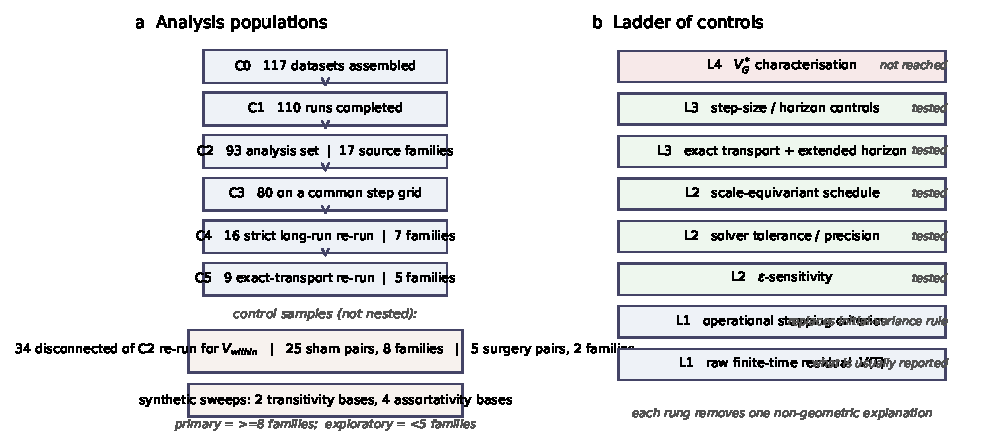
\includegraphics[width=0.86\textwidth]{Fig1_analysis_flow.pdf}
\caption{\textbf{Analysis populations and the ladder of controls.} \textbf{a}, Analysis populations. Nested subsets of the corpus, named
C0--C5 and used consistently throughout; each box gives the number of networks
and, where inference is drawn, the number of independent source families. The
strict re-run C4 is a cost-stratified convenience sample (all 16 below
$0.76$~s per step, cost ranks 3--22 of 113), not a random sample, and no
prevalence claim is made from it. Of C2, 34 networks are disconnected and all
were re-run under the within-component estimator (Supplementary Table~S3);
the 25 sham pairs and 5 surgery pairs are separate control samples drawn from
the same corpus.
\textbf{b}, The ladder of controls. Each rung removes one non-geometric
explanation for an observed residual, from the raw finite-time value (L1) to
the exact-transport, long-horizon and step-size controls that approach L3.
The top rung, characterisation of $V_G^*$ (L4), is not reached: no control in
this paper bounds the geometric infimum.
}
\label{fig:1}
\end{figure}

\begin{figure}[t]
\centering
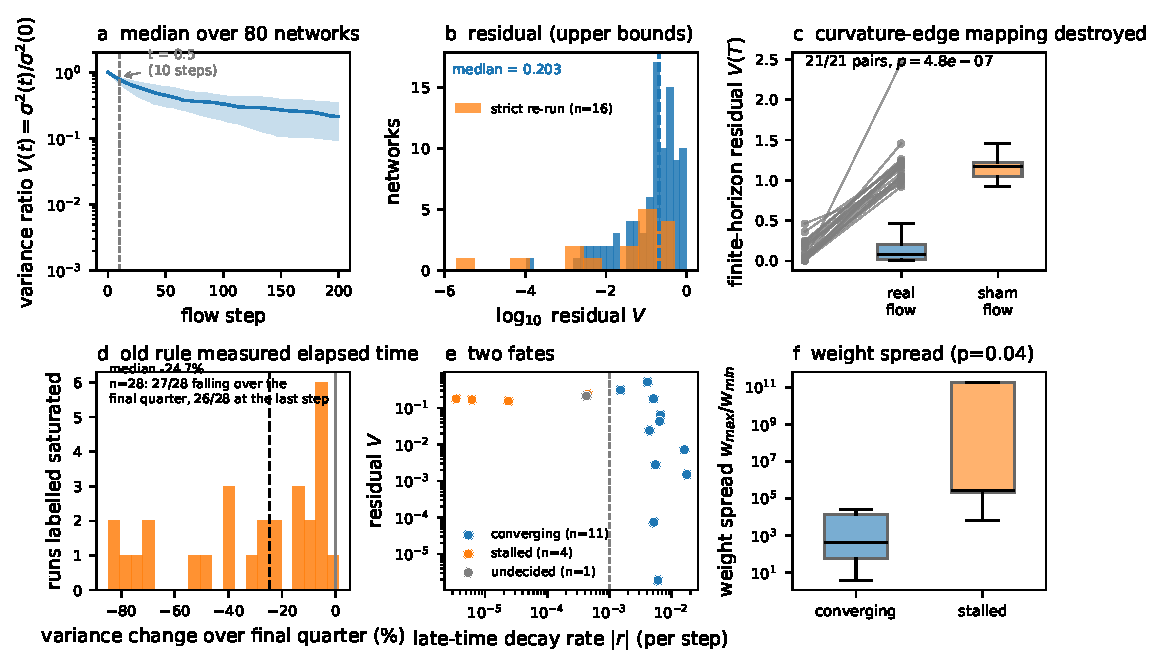
\includegraphics[width=\textwidth]{Fig2_homogenization_and_control.pdf}
\caption{\textbf{The stopping rule decides the story, and the runs separate
into two finite-horizon relaxation patterns.} \textbf{a}, Median (line)
and interquartile range (band) of the variance ratio $V(t)$ over 80 networks
with usable trajectories, on a common step grid; the 10-step transient used in
earlier work sits at $0.78$. \textbf{b}, Residual at the end of the run for
the whole corpus ($n=93$, terminal finite-horizon residuals) and for the 16 networks re-run under
the corrected criterion (orange). \textbf{c}, Sham control: paired residuals
with the curvature--edge mapping randomly permuted each step ($n=25$ pairs,
sham higher in $24/25$, $p=7.7\times10^{-7}$; $21/21$ on the pre-specified
subset). \textbf{d}, Variance change over the final quarter of the 28 runs the
old rule labelled ``saturated'': all but one were still falling. \textbf{e},
Residual against the late-time decay rate for the strict re-run, separating
Pattern~I (blue) and Pattern~II (orange); the dashed line marks a
descriptive $10^{-3}$ per step rate, used only to make the two bands visible,
and it is not a decision boundary. \textbf{f}, Edge-weight
spread at the end of the run by pattern (Mann--Whitney $p=0.04$ at the
network level; family cluster-bootstrap interval for the median
difference $2.85$ decades, $[2.64, 5.25]$). Two of the four
Pattern~II networks are disconnected, and for both the
residual is a between-component term (Table~\ref{tab:components}).}
\label{fig:2}
\end{figure}

\begin{figure}[t]
\centering
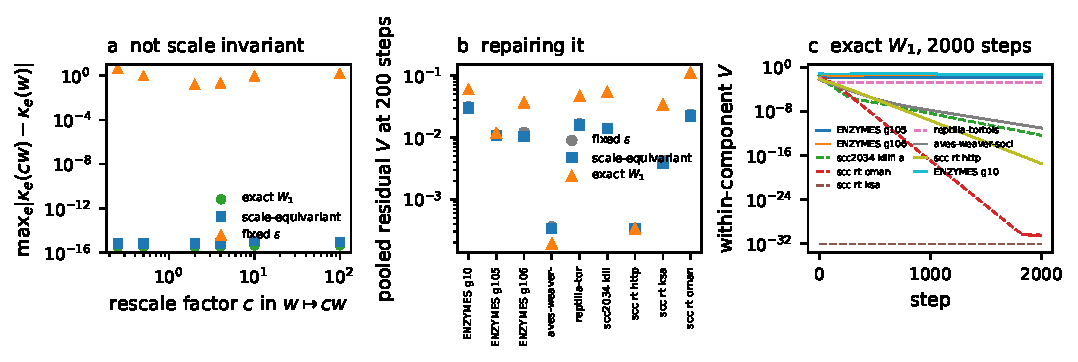
\includegraphics[width=\textwidth]{Fig3_regularisation.pdf}
\caption{\textbf{The regularised curvature is not scale invariant, and repairing it does not remove the residual.} \textbf{a}, Maximum curvature change under a global rescale $w\mapsto cw$, over nine networks, two phases and six rescale factors. Exact $W_1$ transport and the scale-equivariant schedule are invariant to machine precision; the fixed-$\varepsilon$ solver used throughout the paper is not, by up to $3.9$ in a curvature whose range is $O(1)$. \textbf{b}, Residual at a matched horizon of $200$ steps under the three estimators. \textbf{c}, Exact transport, no regularisation, $2{,}000$ steps, within-component variance. Solid lines are connected graphs, dashed lines disconnected ones. Five of the nine fall below $10^{-11}$---two connected (still falling at the last step) and three disconnected, whose pooled variance stays at $0.03$--$0.11$. Four do not: three connected ENZYMES graphs hold $1.2\times10^{-2}$ to $5.2\times10^{-2}$, two of them flat to $<0.2\%$ over the final $800$ steps while their weight span reaches $10^{26}$--$10^{28}$, and one disconnected graph holds $1.4\times10^{-3}$.}
\label{fig:3}
\end{figure}

\begin{figure}[t]
\centering
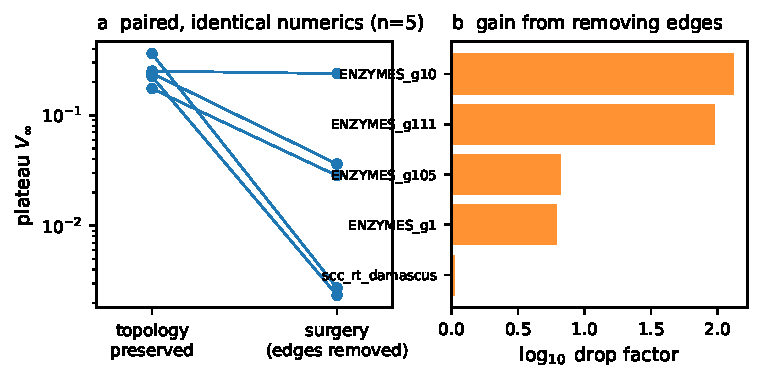
\includegraphics[width=0.8\textwidth]{Fig4_surgery.pdf}
\caption{\textbf{Relaxing the edge-set constraint largely removes the
residual.} \textbf{a}, Paired residuals with identical numerics; the
constraint-relaxation arm removes only edges whose curvature stays above
tolerance ($4$--$14$ edges of $41$--$84$, bridges protected). Relaxed arm lower
in $5/5$ pairs ($p=0.031$). \textbf{b}, Drop factor per pair (median
$6.6\times$, maximum $132\times$). The intervention is outcome-informed---edges
are selected by the curvature the flow produced---so this is a
constraint-relaxation control, not a causal demonstration.}
\label{fig:4}
\end{figure}

\begin{figure}[t]
\centering
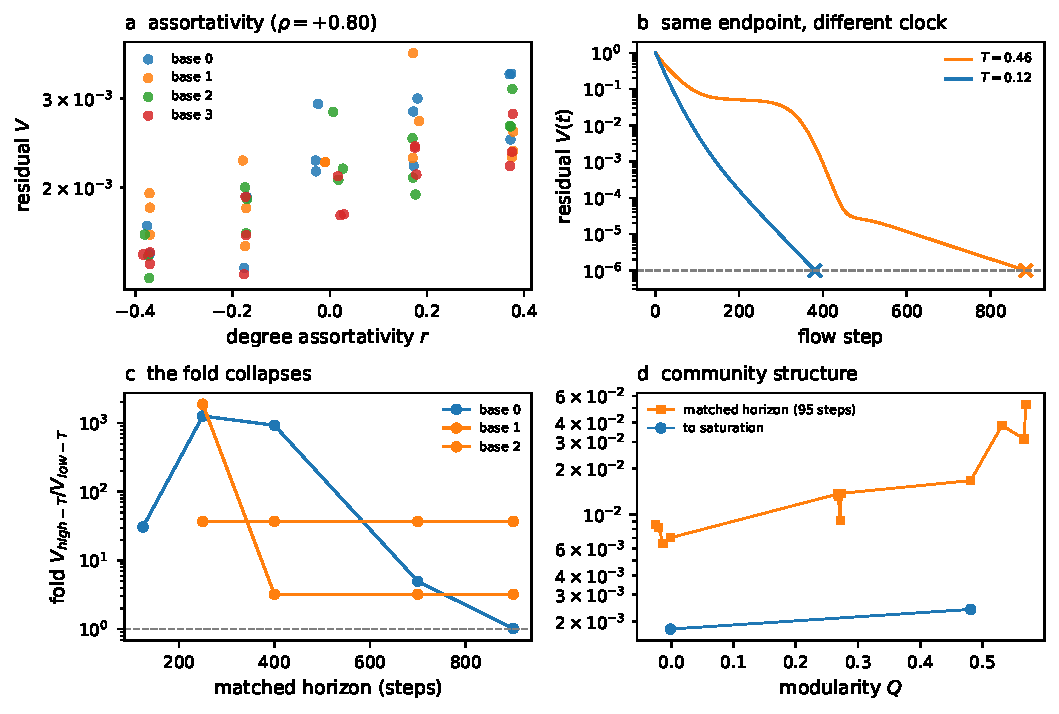
\includegraphics[width=\textwidth]{Fig5_mechanism.pdf}
\caption{\textbf{Transitivity changes the clock, not the destination;
community structure changes neither.} Degree sequences are held exactly fixed
throughout. \textbf{a}, Residual versus manipulated assortativity ($n=60$
saturated cells, 4 bases). \textbf{b}, Both arms of one base graph followed to
a terminal state: raising transitivity from $0.12$ to $0.46$ leaves the
endpoint unchanged---both arms reach the operational threshold $V=10^{-6}$
(crosses at steps $381$ and $884$)---but multiplies the time to get there by
$2.3$; the dashed line is the floor. \textbf{c}, The fold between the two arms
is a transient, not a plateau difference: $31\times$ at $125$ steps,
$1.3\times10^{3}$ at $250$, $9.3\times10^{2}$ at $400$, $5.0$ at $700$ and
$1.02$ at $900$ (base 0; bases 1 and 2 shown to their horizons).
\textbf{d}, Community structure: strong at a matched 95-step horizon
($6.1\times$) but only $1.35\times$ at saturation---matched-horizon
comparisons mistake slower convergence for a higher plateau.}
\label{fig:5}
\end{figure}

\begin{figure}[t]
\centering
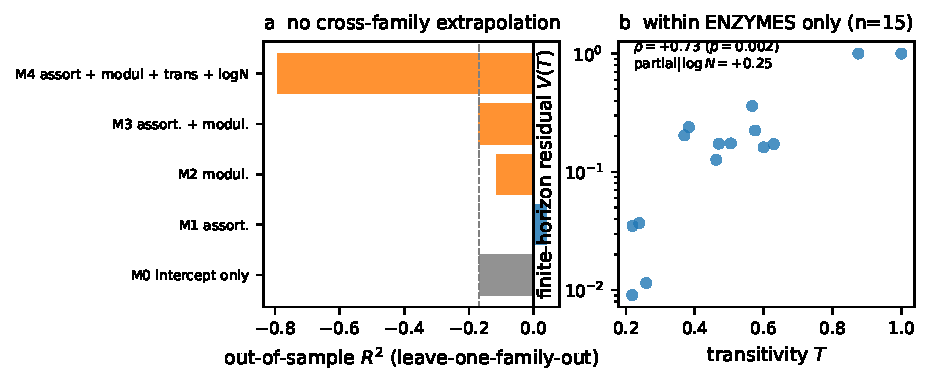
\includegraphics[width=0.8\textwidth]{Fig6_predictability.pdf}
\caption{\textbf{The structure-to-residual mapping does not transfer across
families.} \textbf{a}, Leave-one-family-out out-of-sample $R^2$; only assortativity
rises marginally above the intercept baseline (dashed), and none of the
models has usable predictive power. \textbf{b}, Within
the largest family (ENZYMES, $n=15$ converged) the plateau correlates with
transitivity ($\rho=+0.73$) but the correlation collapses once size is
controlled (partial $\rho=+0.25$, $p=0.37$). \textbf{c}, Family-level cluster-bootstrap 95\% intervals for the corpus correlations over 41 units and 11 families: the assortativity association survives clustering, the transitivity one does not, and the rate--residual interval includes zero.}
\label{fig:6}
\end{figure}

\begin{figure}[t]
\centering
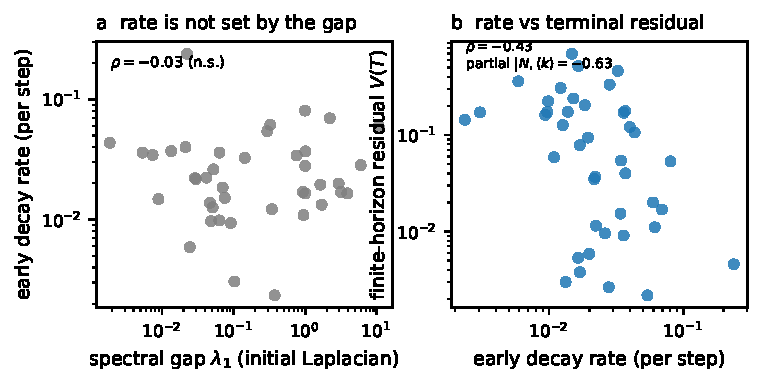
\includegraphics[width=0.8\textwidth]{Fig7_dynamics.pdf}
\caption{\textbf{Speed and depth are coupled; the spectral gap is not the
clock.} \textbf{a}, Early decay rate versus initial Laplacian spectral gap
across 41 units ($\rho=-0.03$, n.s.; cluster-bootstrap interval [-0.43,+0.39]); the gap does not set the rate.
\textbf{b}, Faster decay reaches a lower plateau ($\rho=-0.43$; partial
$\rho=-0.63$, controlling size and mean degree); the family cluster-bootstrap interval [-0.68,+0.16] includes zero, so we do not claim the association at family level.}
\label{fig:7}
\end{figure}

\begin{figure}[t]
\centering
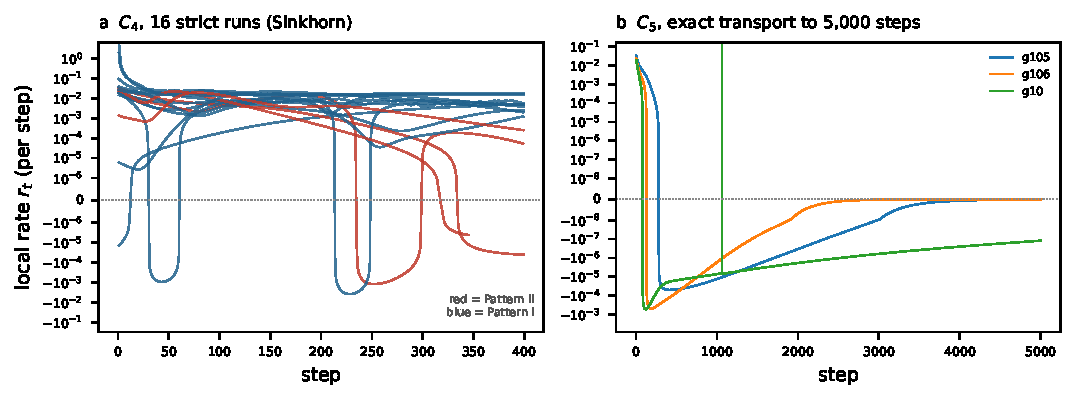
\includegraphics[width=\textwidth]{Fig8_relaxation_rate.pdf}
\caption{\textbf{The relaxation-rate trajectory, rather than a
classification.} \textbf{a}, Local relaxation rate
$r_t=-\log(V_t/V_{t-1})$ for the $16$ runs of population $C_4$; $r_t>0$ is
decay, $r_t\approx0$ a plateau, $r_t<0$ a rebound ($234$ of $6{,}052$
increments, $3.9\%$, are rebounds). Two bands are visible---one above
$10^{-3}$ per step and one decaying towards $10^{-5}$---but runs cross between
them, so the bands are a description of the horizon, not of the limit. Red:
near-plateau at the horizon; blue: still relaxing. \textbf{b},
The two connected ENZYMES networks and a third under exact transport to
$5{,}000$ steps: $r_t$ falls below $10^{-7}$ per step and stays there, while
the weight span grows to $10^{71}$---no appreciable decay over the extended
horizon.}
\label{fig:8}
\end{figure}

\end{document}
